\documentclass[a4paper,12pt]{report}
\usepackage[utf8]{inputenc}
\usepackage[T1]{fontenc}
\usepackage{xspace}
\usepackage[francais]{babel}
\usepackage[]{algpseudocode}
\usepackage[hidelinks]{hyperref}
\usepackage{graphicx}

% Title Page
\title{Rapport technique \\Mini Projet : Le jeu du carré, IA joueuses}
\author{Ange Jennyfer NGUENO FOKAM - 170840\\Julien PETRIGNET 217307\\Titouan FREVILLE - 217821\\Sara EL AICHI 226328}

% Document start
\begin{document}
% Title :O
\maketitle
% contents
\tableofcontents
% captations
\listoffigures

% R\'esum\'e
\begin{abstract}
Le projet IA joueuses pour le jeu du carré à pour but de répondre au sujet de 4AIT de l'école Supinfo, promotion 2018. L'objectif du projet est de réalisé aux moins deux intelligences artificielle capable de jouer au jeu du carré. Les intelligences propos\'ees devront \^etre capable de jouer entre elle ou contre un joueur ext\'erieur. \\
\\
A partir de cet \'enonc\'e, plusieurs solutions s'offrent \`a nous. Pour pouvoir r\'epondre le mieux aux probl\`emes, il nous faut tout d'abord analyser le jeu s\'electionner afin de d\'eterminer son type (d\'ecision, for\c{c}age, anticipation, calcul, r\'eaction, ...). Nous pourrons alors nous interroger sur les diff\'erentes IA proposable puis sur les langages utilisables afin de s\'electionner le plus intéressant pour nous.
\\
Ce rapport \`a pour but de pr\'esenter toute la d\'emarche de r\'eflexion que nous avons eu afin de prendre une d\'ecision nous permettant de r\'esoudre le probl\`eme de la fa\c{c}on la plus intéressante.
\end{abstract}

% ------------------------------------------------------------- PRESENTATION GENERALE JEU -------------------------------------------------------------  %
\part{Le jeu, pr\'esentation et compr\'ehension}

\chapter{Historique, principe de base, type}
Le jeu du carr\'e est un jeu d\'ecris en 1889 pour la premi\`ere fois par Edouard Lucas, math\'ematicien. Le principe du jeu est tr\`es simple, et nécessite peu de mat\'eriel. Le but est de cr\'eer des forme carr\'e. Pour cela, chaque joueur va a tour de r\^ole tracer un segment sur un quadrillage permettant de repr\'esenter un c\^ot\'e pour un future carr\'e. Le jouer ayant ferm\'e le plus de carr\'e remporte la partie.

\section{Type de jeu}

Le jeu des petits carr\'es est un jeu de r\'eflexion. Il fonctionne comme le jeu de dame, dans le sens ou, lorsque le jeu est ma\^itriser, l'objectif devient de forcer le jouer adverse a fermer un certain nombre de carr\'e pour pouvoir en r\'ecup\'erer plus par la suite. C'est donc un jeu de for\c{c}age et de d\'ecision. Fonctionnant sur des formes g\'eom\'etrique, il va donc se concentr\'e sur la capacit\'e \`a lire le plan repr\'esenter par la grille et \`a venir correctement enfermer l'adversaire dans une situation de fermeture perdante. Nous allons donc chercher \`a permettre \`a nos IA une bonne compr\'ehension de l'occupation de l'espace, et une bonne lecture du plan grillag\'e.

\section{Compr\'ehension}

D\'etaillons maintenant la strat\'egie principale du jeu.\\
Le jeu se base donc sur la g\'eom\'etrie et plus particuli\`erement les formes rectangulaires, et les carr\'es. La premi\`ere phase du jeu va avoir pour objectif de cr\'eer des zones de \og{}non droit\fg{} tel que si un joueur place un trait dans cette zone, il donne une grande quantit\'e de points \`a son adversaire. Ensuite, chaque joueur va devoir essayer d'agrandir sa zone de non droit et en \og{}poss\'eder\fg{} une depuis la qu'elle il r\'ecup\'erera plus de points que son adversaire. L'objectif est donc de cr\'eer un couloir (appeler plus g\'en\'eralement \og{}serpent\fg{} en raison de sa forme) longiligne puis de forcer l'adversaire \`a jouer en bordure de ce couloir tel que d\`es qu'il ferme un carr\'e dans cette zone, le joueur r\'ecup\`ere plus de point que lui. \\
Cette strat\'egie essentiel est toutefois complexe, et n'est pas ce que les joueurs seront capable de produire en premier. Afin de proposer des IAs \'equilibr\'ees,  il nous faudra donc une IA incapable de pr\'evoir/comprendre ce Fonctionnement. \\
Nous pouvons d\'ej\`a entrevoir deux syst\`eme pour concevoir nos IA: une IA simpliste compl\'etant la grille et fermant les carr\'es d\`es que possible, et une IA plus complexe g\'erant la notion basique de serpent sans anticiper sur les coups \`a venir.
% -----------------------------------------------------------------------------------------------------------------------------------------------------  %
% ------------------------------------------------------------- PRESENTATION IA  ----------------------------------------------------------------------  %
\part{Intelligence Artificielle, let's play}
\chapter{D\'efinition des IA}

Dans la partie pr\'ec\'edente, nous avons parl\'e de plusieur IA possible, plus pr\'ecis\'ement, nous avons introduit deux IA simple. Nous allons ici continuer ce travail afin de red\'efinir les IAs et les compl\'eter.


% ---- IA 0 ------------------------------------------------------------------------
\section{IA - Base. Niveau 0}

La premi\`ere IA que nous allons d\'ecrire servira de base \`a toutes les IAs suivantes. C'est l'IA la plus simple que l'on puisse faire pour obtenir un r\'esultat interressant, et ce n'est pas pleinement une IA dans le sens ou elle va simplement automatiser un processus de traitement de donn\'ee. \\
L'unique objectif de cette IA est d'\^etre capable de jouer au jeu.

\subsection{Principe}

L'IA basique a donc pour objectif simple de pouvoir placer correctement les liasons sur la grille, et \^etre capable de prendre des points. Pour ce faire, elle va se contenter de placer les liaisons hors carr\'e (des liaisons entre deux somets sont c\^ot\'e) de fa\c{c}on al\'eatoire sur la grille. Puis elle compl\'etera les carr\'es ayant un c\^ot\'e. Une priorit\'e absolue est donn\'e pour fermer les carr\'es, ce qui im\`plique que l'IA ferme de fa\c{c}on syst\'ematique les carr\'es visible jouable \`a son tour. Elle est incapable de calculer le revenu (en point d'une de ses actions).

\subsection{Heurisitque}

Cette IA a donc besoin de peu de connaissance, et peux de processus. Ces connaissances seront par la suite pr\'esente dans toutes les IAs. \\

\begin{itemize}
 \item Capable de relier deux sommets correctement
 \item Capable de lire la grille
 \item Capable de trouver les carr\'es fermable
\end{itemize}

Ces trois \'el\'ements sont suffisant pour que cet IA puisse fonctionner.

\subsection{Algorithmes}

Pour la d\'efinition de l'algorithme, nous abstrayon la lecture et les types de donn\'ees par la fonction : lireGrille(grille) dont on suppose le typage connue, et qui nous renvoie les informations voulues. \\
L'algoritmhe que nous allons utiliser pour la premi\`ere IA est simpliste. Il utilise la fonction de lecture lireGrille pour r\'ecup\'er\'e soit un carr\'e soit une liaison vide. Nous allons d\'efinir de fa\c{c}on abstraite la fonction lireGrille capable de renvoyer ces information puis l'algorithme de l'IA. \\
\begin{algorithmic}
\Function{lireGrille}{$grille$}
	\State $case \gets currentCase$
	\ForAll{$case$ in $reachableCase$}
		\If {$case$ is $closable$}
			\State \Return $case$
		\Else
			\If {$grilleEnd$}
				\State \Return $randomCase$
			\EndIf
		\EndIf
	\EndFor
\EndFunction
\\
\Function{ia0}{}
	\While {$true$}
		\State $caseToPlay\gets$lireGrille($grille$)
		\If {$caseToPlay$ is $closable$}
			\State closeCase()
			\State countPoints()
		\Else
			\State drawCaseSegment()
		\EndIf
		\State waitOverPlayer()
	\EndWhile
\EndFunction
\end{algorithmic}
Les fonctions abstraite drawCase, closeCase, countPoints et waitOverPlayer sont considir\'e comme de compl\'exit\'e neutre et instantan\'ee par rapport aux autres fonctions. Leur utilisation est \'evidente ainsi que ce qu'elle font.

\subsection{Complexit\'e}

\subsubsection{Spaciale}

Assez peu de compl\'exit\'e spaciale pour cette algorithme. Une variable est utilis\'e pour la grille, une pour stocker la case en cours d'analyse, une pour le score et une pour attendre l'autre jouer. Soit 4 variable simultan\'ees. La plus part de ces variables contiennes une valeur courte pouvant \^etre stocker faiclement et occupant tr\`es peu d'espace. La grille sera un peu plus longue, et son poid sera d\'ependant de la taille de celle-ci ainsi que du choix de repr\'esentation. On peut donc dire que la complexit\'e spaciale $CS$ est \'equivalente \`a la compl\'exit\'e spaciale de la grille $CSG$. L'occupation de la m\'emoire est donc tr\`es raisonable et, elle augmentera de fa\c{c}on lin\'eaire en fonction du nombre d'\'el\'ement de la grille. 

\subsubsection{Temporelle}

La compl\'exit\'ee temporelle de cette algorithme est assez facile a calculer: \\
$CT_{ia0}$($n$) = O($CT_{lireGrille}$($n$)$*$4$n$) = O($n*$4$n$)=O(4$n^2$) = O($n^2$), o\`u $n$ est le nombre de case de la grille. \\
Cette algorithme est donc tr\`es peu optimis\'e, est long a s'\'exut\'e. Son temps d'\'ex\'ecution augmlente en fonction du carr\'e du nombre de case. Il devient donc rapidement au dela d'un temps d'attente supportable. Cependant, ce temps d'\'ex\'ecution est globale sur toute l'\'exution de l'IA, c'est a dire, globalement, si nous faisons s'affronter les deux IAs, cette augmentation de temps est valalble. Dans une utilisation en joueur contre IA, nous pouvons r\'eduire la compl\'exit\'e de l'\'ex\'ecution a la complexit\'e de jouer un tour, le joueur n'ayant qu'a attentendre le coup suivant de l'IA a chaque \'etape. Nous avons alors une compl\'exit\'e lin\'eraire en fonction du nombre d'\'el\'ement de la grille, l'IA ne lisant qu'une seule fois la grille compl\`ete \`a chaque tour de jeu.

Cette IA est donc relativement rapide en terme d'attente pour le joueur entre chaque tour. Par contre, elle ne devrait pr\'esenter aucune difficult\'e apr\`es quelque partie. Il est \'egalement \`a not\'e que le temps sera un facteur beaucoup plus limitant que l'espace pour cette IA. 

% ---- IA 1 ------------------------------------------------------------------------
\section{IA - Premi\`eres armes. Niveau 1}

D\'eveloppons maintenant une IA utilisant les structures de serpents introduite en premi\`ere partie. 

\subsection{Principe}

Cette seconde IA se base sur les m\^emes connaissances que l'IA pr\'ec\'edente. Cependant, nous allons modifier les r\`egles de placement des liaisons et ajouter la capacit\'e \`a compter les points. Ainsi, plut\^ot que de placer de fa\c{c}on al\'eatoire des c\^ot\'es, cette nouvelle IA va chercher \`a cr\'eer des serpents et des coridors. Par cons\'equents, elle va en priorit\'e placer un segment au bout d'un autre segment en cherchant a relier deux sommets sp\'ecifiques. Le choix de liaisons entre deux sommets se fait sur la quantit\'e de points r\'ecup\'erables \`a la fermeture du serpent, cette valeur devant \^etre maximis\'ee. Lorsque l'IA \`a la possibilit\'e de clore un serpent, elle va s'interroger sur la quantit\'e de points qu'elle va gagner en le fermant par rapport \`a la quantit\'e de point que l'adversaire peut r\'ecup\'erer. Si le rapport est positif, elle fermera syst\'ematiquement le serpend

\subsection{Heurisitque}

Notre seconde IA a donc besoin de nouvelle connaissance, bien qu'elle reste tr\`es simpliste.

\begin{itemize}
 \item Capable de choisir le meilleur segment d'un serpent
 \item Capable de compter les points gagnables par chaque partie dans une configuration connue
\end{itemize}

Il lui faut donc deux nouvelles connaissance pour fonctionner correctement.

\subsection{Algorithmes}

\begin{algorithmic}
\Function{addMove}{$case$, $side$, $snakeList$}
	\State Match $snakeList$ with
	\State $Empty$ $\rightarrow$ [([($case$, $side$)],1)]
	\State ($snake$, $val$) :: $q$ $\rightarrow$
		\If {inSnake $case$ $snake$}
			\If {member $case$ $snake$}
				\State (($case$, $side$)::$snake$, $val$)::$q$
			\Else
				\State (($case$, $side$)::$snake$, $val$+1)::$q$
			\EndIf
		\Else
			\State $t$::addMove $case$ $side$ $q$
		\EndIf
\EndFunction
\\
\Function{move}{$grille$,$snakeList$}
	\State Match $snakeList$ with
	\State $Empty$ $\rightarrow$ let $case\gets$randomCase() in addMove $case$ randomInt(0,3) $snakeList$
	\State ($snake$, $val$) :: [] $\rightarrow$
		\If {isClosableSnake($snake$)}
			\State closeSnake($snake$)
		\EndIf
	\State ($snake$, $val$) :: ($snake2$, $val2$)::$q$ $\rightarrow$
		\If {isClosableSnake($snake$)}
			\State closeSnake($snake$)
		\Else
			\If {closableWith($snake$, $snake2$)}
				\State force($snake2$)
			\Else
				\State move($grille$,$q$)
			\EndIf
		\EndIf
\EndFunction
\\
\Function{force}{$snake$}
	\If {isClosableSnake($snake$)}
		\State randomCase($snake$)
	\EndIf
	\State let (c1, c2) = snakeEnd($snake$) in
	\If {closedSides(c1) < 3}
		\State addSnakeSide(c1)
	\Else
		\If {closedSides(c2) < 3}
			\State addSnakeSide(c2)
			\Else randomCase($snake$)
		\EndIf
	\EndIf
\EndFunction
\\
\Function{ia1}{$grille$,$snakeList$}
	\State move($grille$,$snakeList$)
	\State waitOverPlayer()
	\State ia1($grille$, $snakeList$)
\EndFunction
\end{algorithmic}
Les fonctions non d\'efinis sont consid\'er\'e comme abstraite et connue (car d\'ependante du type de donn\'ees) et soit en temps r\'eel soit sur une compl\'exit\'e maximale de $n$. 

\subsection{Complexit\'e}

\subsubsection{Spaciale}

Cette s\'erie d'algorithme utilise plus de place que le pr\'ecendent. Une variable suppl\'ementaire doit \^etre utiliser pour stocker la liste des serpents. La compl\'exit\'e de la liste de serpent d\'ependant de celle de la grille, et on peut dire que dans le pire des cas, elle sera de : $CSG*CSG$. En l'ajoutant \`a la compl\'exit\'e pr\'ec\'edente, on a que $CSA1=O(CSG+CSG^2)=CSG^2$. Aussi, dans le pire des cas, l'occupation de l'espace augmente exponentiellement vis \`a vis de la taille de la grille. Cependant, le cas ou chaque \'el\'ement de la grille se retrouve dans chaque serpent possible est quasiment impossibe, sauf mal utilisation des fonctions de cr\'eations des serpents. On peut m\^eme dire que dans un cas id\'eale, ou il n'existe qu'un serpent, la compl\'exit\'e spaciale sera lin\'eaire en fonction du nombre d'\'el\'ement de la grille. Par cons\'equent, en moyenne, la compl\'exit\'e spaciale de la fonciton sera en moyenne logarithmique, aussi, on peut supposer que l'espace pris par la fonction augmentera \'enormement en fonction du nombre d'\'el\'ement dans la grille pour des petites tailles puis aura tendance a se stabilis\'e pour des grilles de tr\`es grande taille. 

\subsubsection{Temporelle}

Les compl\'exit\'es sont donn\'ees pour les pires cas. Soit $n$ le nombre de case de la grille.

$CT_{addMove}$ = O$(n*n)$ = O$(n^2)$ \\
$CT_{force}$ = O$(CT_{isClosableSnake}+CT_{snakeEnd}) = $O$(n+n) = $O$(n)$ \\
$CT_{move}$ = O$(CT_{isClosableSnake}+CT_{closeSnake}+CT_{closableWith}+CT_{force})*n$ = O$(n+n+n+n)*n$ = O$(n^2)$


La compl\'exit\'e temporelle au pire est crois donc exponentiellement en fonction du nombre d'\'el\'ement dans la grille. Cependant, le cas ou chaque \'el\'ement de la grille donne un serpent contenant tous les \'el\'ements de la grille ne devrait pas arriv\'e dans un contexte d'utilisation normale. On peut approxim\'e la compl\'exit\'e moyenne a $n*log(n)$ en prenant en compte le fait que la liste des serpents sera tri\'e \`a chaque modification afin de conserver le serpent donnant le plus de point en prem\`ere position. Nous nous retrouvons alors dans la m\^eme situation que pour la compl\'exit\'e spaciale. 

Globalement, c'est algorithme sembe donc plus lourd que l'algorithme pr\'ec\'edent pour un joueur contre joueur. Cependant, pour une grille tr\`es grande, il va tendre \`a se rapprocher de l'algorithme de niveau 0 en vitesse et en occupation de l'espace. Il est donc plus int\'eressant pour un jeu standart avec des personnes ayant une compr\'ehension correcte du jeu, mais cherchant un adversaire relativement simple \`a battre. Il est d'autant plus int\'eressant que des joueurs cherchant un certain challenge devrait joueur sur des grilles relativement grande, et par cons\'equent, r\'ev\'eler l'efficacit\'e de cette algorithme proposant un bon \'equilibre entre compl\'exit\'e de jeu et temps de jeu.

% ---- IA 2 ------------------------------------------------------------------------
\section{IA - La connaissance. Niveau 2}

Pour le joueur, l'IA 1 va \^etre plus complexe a vaincre par sa capacit\'e \`a choisir l'option avec meilleur gain. Cependant, elle reste extr\`emement simple \`a vaincre car tr\`es sensible au forcing. Ce qui nous am\`ene \`a une nouvelle IA. 

\subsection{Principe}

L'IA que nous allons introduire ici est l'IA la plus compl\`ete que l'on puisse faire pour un jeu. Elle est simple \`a comprendre, mais extr\`emement difficile \`a battre. Elle consiste \`a g\'en\'erer l'int\'egralit\'e des \'evolutions possibles dans une grille de la grille vide a la grille pleine. Elle connait alors toutes les configurations possibles \`a chaque instant de la partie et vas toujours choisir le placement lui donnant le plus de condition de victoire \`a chaque instant.

\subsection{Heurisitque}

Notre troisi\`eme IA a donc besoin d'une seule chose en plus de l'IA 0: la connaissance de toutes les configurations. Elle n'a plus besoin de savoir compter les points puisque elle sait qu'elle coup l'am\`ene \`a la victoire. Elle n'a plus non plus besoin de savoir construire des serpents. Bref, il lui faut juste revenir aux connaissance de bases et cr\'eer l'arbre de connaissance correspondant \`a la grille demand\'e par le joueur.

\subsection{Algorithmes}

\begin{algorithmic}
\Function{initTreeMove}{$grille$,$moveTree$}
	\State Match $grille$ with
	\State $Empty$ $\rightarrow$ $EmptyTree$
	\State $case$::$resteGrille$ $\rightarrow$
		\If {isClosed($case$)}
			initTreeMove($q$, $moveTree$)
		\Else
			\For {$i$ from $0$ to $3$}
				\State let $newGrid$ = play($case$,$i$,$grille$) in
				\State let $moveTreeFrom$ = initTreeMove($newGrid$, $EmptyTree$) in
				\State let $newMoveTree$ = addTree($moveTreeFrom$, $moveTree$) in
				\State initTreeMove($resteGrille$, $newMoveTree$)
			\EndFor
		\EndIf
\EndFunction
\\
\Function{selectPlay}{$treeMove$}
	\State Match $treeMove$ with
	\State $EmptyTree$ $\rightarrow$ $EndGame$
	\State $(Racine, lFils)$ $\rightarrow$ playWinner($lFils$)
\EndFunction
\\
\Function{playWinner}{$listTreeMove$}
	\State Match $listTreeMove$ with
	\State $Empty$ $\rightarrow$ ($EmptyTree$,0)
	\State $t$::$Empty$ $\rightarrow$ ($t$, score($t$)
	\State $t$::$q$ $\rightarrow$ let ($currentWinner$, $currentScore$) = playWinner($q$) and $thisScore$ = score($t$) in
		\If {$thisScore$ > $currentScore$}
			\State ($t$, $thisScore$)
		\Else
			\State ($currentWinner$, $currentScore$)
		\EndIf
\EndFunction
\\
\Function{ia2}{$moveTree$}
	\State let $newTree$ = playWinner($moveTree$) in
	\State let $playerTree$ = waitOverPlayer($newTree$) in
	\State ia2($playerTree$)
\EndFunction
\end{algorithmic}
Les fonctions $score$ et $play$ sont abstraite de compl\'exit\'e simple (O(1)). La fonction $addTree$ n'est pas pr\'esenter ici car d\'ependante de la mod\'elisation des donn\'ees, elle sera cependant assez classique (lire l'arbre jusqu'a arriver \`a la place de l'\'el\'ement \`a ajouter et \'equilibr\'e si n\'ecessaire).

\subsection{Complexit\'e}

\subsubsection{Spaciale}

La complexit\'e spaciale de cette fonction est essentiellement li\'ee \`a la taille de l'arbre des coups, et \`a sa cr\'eation. Nous pouvons limiter l'impact en m\'emoire en utilisant de la r\'ecursivit\'e terminale au lieu de la r\'ecursivit\'e standart, permettant ainsi de ne plus puiser dans les ressources de la RAM. Cependant, le programme demandera tout de m\^eme de stocker la grille compl\`ete et l'arbre des possibles complet. On peut dire que la complexit\'e spaciale globale est li\'e \`a la compl\'exit\'e spaciale de la grille ainsi: $CSGlobale=CSGrille*(n!)$ ou n est le nombre de case. Nous pouvons en conclure que, si nous n'appliquons pas de r\'ecursivt\'e terminale, nous allons tr\`es rapidement d\'epasser la m\'emoire d'un ordinateur standart, car pour chaque appel r\'ecusif, nous allons stocker un arbre de taille $CSGlobale$. Le nombre d'appel r\'ecursif augmentant avec la taille de la grille de fa\c{c}on lin\'eaire, nous pouvons dire que l'algorithme occupe une large place dans la m\'emoire en r\'ecursif stantdart, et il est certain qu'une r\'ecursivit\'e terminale permettrait de compenser cette failblesse. Cependant, au vue des performances actuelle des ordinateur, nous pouvons l'impl\'ementer en r\'ecursif non terminale en limitant la taille de la grille, et en se basant sur des tailles \og{}standart\fg{} de l'ordre de $8*8$ par exemple.

\subsubsection{Temporelle}

Dans cette configuration, l'essentielle de la compl\'exit\'e temporelle est li\'e \`a la g\'en\'eration de l'arbre des possibles. En effet, les fonctions $selectPlay$, $playWinner$ et $ia2$ auront au pire une compl\'exit\'e de $n$. 

La compl\'exit\'e de la fonction de g\'en\'eration des coups est li\'e \`a la compl\'exit\'e d'ajout d'un \'el\'ement dans l'arbre. N'ayant pas pr\'esenter l'algorithme d'ajout (li\'e \`a la mod\'elisation des donn\'ees), nous notterons $CT_{ajoutArbre}$ sa valeur exacte, on peut cependant l'approxim\'e \`a $n*log(n)$ \'etant donn\'e la structure d'arbre et en anticiapant le fait que l'arbre ne sera pas \'equilibr\'e via une fonction sp\'ecifique (\'etant donn\'e son objectif), mais qu'il devrait \^etre naturellement \'equilibr\'e par le concept de jeu.

Ainsi, la compl\'exit\'e de la fonction d'ajout sera : 

$CT_{initTreeMove}$ = O($(4*CT_{ajoutArbre}*n)$) = O($CT_{ajoutArbre}^n$) ~ O($(n*log(n))*n$) ~ O($n^2*log(n)$) > O($n^2$)

Pour cette algorithme, la g\'en\'eration de l'arbre des possibles, et donc l'attente avant le lancement du jeu, va augmenter de fa\c{c}on exponentielle, c'est \`a dire que plus la grille va \^etre grande, plus le joueur devra attendre avant de pouvoir commencer \`a jouer. Cependant, le choix d'un coup par l'odinateur augmente de fa\c{c}on lin\'eaire, car il lui suffit de trouver le bon \'el\'ement dans la liste des possibilit\'e suivant l'\'etat actuelle de jeu. Cette liste ne pouvant d\'epasser le nombre d'\'el\'ement pr\'esent dans la grille, et le nombre d'\'el\'ement possible \'etant r\'eduis \`a chaque \'etape (puisqu'il y a de moins en moins de case jouable), on peut affirmer que l'IA devrait \^etre de plus en plus rapide \`a jouer.

Pour cette derni\`ere IA, nous avons affaire \`a une intelligence tr\`es difficile \`a battre. Cependant, le processus d'initialisation du jeu et de l'IA va \^etre extr\`emement lourd et long. Elle reste cependant interressante pour des joueurs cherchant un challenge \'enorme, bien qu'il ne faille attendre un certain temps avant le d\'ebut de la partie. Il est possible de gagner du temps en g\'en\'erant au pr\'ealable des mod\`ele de grille existant et leurs arbres de coups. Au quel cas, si l'utilisateur choisis une grille connue, le processus de cr\'eation n'est plus n\'ecessaire, et le jeu sera en apparence aussi rapide que pour l'IA 0. 



% ------------------------------------------------------------- MODELISATION -------------------------------------------------------------  %
\part{Mod\'elisation}

Maintenant que nos futures IA sont d\'efinis, voyons comment mod\'eliser les donn\'ees du probl\`emes.

\chapter{Environement}

L'environement de jeu consiste en un plateau pr\'esentant une grille. C'est sur cette grille que nos viendrons dessiner nos segment. Le plateau globale est de forme rectangulaire, id\'ealement carr\'e. La grille est d\'ecouper en carr\'e, d\'ecomposer en ligne et somment. Plusieur solutions s'offrent alors \`a nous pour repr\'esenter l'environement. Nous pouvons d\'efinir un graphe contenant chaque sommet et les liasions entre eux, en utilisant une variable sur chaque noeud pour pr\'esenter la pr\'esence ou non d'une liaison, ou nous pouvons repr\'esenter chaque sommet de la grille dans une matrice, et utiliser une liste pour stocker les liaisons connue. \\

\section{Tableau}

La repr\'esentation via tableau est la repr\'esentation la plus informatique du probl\`eme, et la plus simple vis \`a vis de la repr\'esentation graphique du probl\`eme. Chaque point de la matrice repr\'esentant un sommet de la grille, il est facile de s\'electionner des sommets puis de les liers dans une liste via un couple.\\
L'avantage de cette m\'ethode est donc la facilit\'e de gestion de la partie graphique du jeu. Cependant, il est alors compliquer de savoir qu'elle c\^ot\'e sont d\'ej\`a tracer. Il est donc plus long de r\'ecup\'erer les informations quand aux corridors et serpents pr\'esent de le jeu, ainsi que de s'assurer que le coup est autoris\'e.

\section{Graphe}

La repr\'esentation via graphe va permettre de compenser la faiblesse du tableau vis \`a vis des c\^ot\'e. Cependant, elle sera moins efficace d'un point de vue graphique. Le graphe a repr\'esenter doit stocker les informations sur la case. Vis a vis de la grille, une cas est un future carr\'e, donc un point. Un point est ferm\'e d\`es que ces 4 c\^ot\'es sont ferm\'e. Un sommet de notre graphe serait alors un triplet contenant le nom de la case (ex: C5), une liste bool\'een correspondant au c\^ot\'e de la case (vrai si ferm\'e, faux sinon par exemple), et une liste contenant au plus quatre \'el\'ement repr\'esentant les noms des cases adjacentes. \\
Nous avons alors une structures qui permet de facilement calculer les points de la carte, de visualiser les structures de corridors et serpents et de g\'erer les liaisons entre les cases. Bien que moi efficace sur le plan graphique, elle est beaucoup plus puissantes pour les algorithmes de r\'esolution et plus rapides. 

\section{Solution choisie}

Nous avons donc choisi la structure de graphe pour mod\'eliser les donn\'ees. L'objectif de notre travail \'etant principalement de cr\'eer des IAs capable de jouer au jeu, et non de permettre a deux joueurs de s'affronter. Nous avons naturellement choisi la solution la plus interressante du point de vue algorithmique. 

\chapter{Information de jeu}

Une fois la repr\'esentation de l'environement choisi (en l'occurence, un graphe), il nous faut mod\'eliser les coups et options de jeu. Encore une fois, il y a plusieur solutions. Cepenant, ici, les diff\'erentes solutions vont plus s'appliquer au choix d'impl\'ementation d'IA qu'a un besoin. En effet, pour l'IA de niveau 0, il n'y a pas besoin de structure particuli\`ere pour symboliser les coups. Une simple lecture du graphe suffit. Les structures sont a d\'efinir pour l'IA de niveau 1 et 2. 

\section{IA 1 - Structure}

La premi\`ere IA a besoin d'une connaissance sp\'ecifique a chaque configuration du graphe : la quantit\'e de points gagnable pour chaque serpent. Cette valeur peut s'obtenir en comptant le nombre de carr\'e pr\'esent dans le serpent. Dans un soucis de vitesse, une liste contenant les diff\'erents serpents ainsi que le diff\'erentiel de points joueur/IA peut \^etre int\'eressante a d\'efinir. Au quel cas, apr\`es chaque coups, cette liste est mise \`a jour. Dans cette liste, un serpent est un triplet contenant le nom de la case de d\'epart, et celui de la case de fin, puis le diff\'erentiel de score (ex: le triplet (A0, A3, 4) repr\'esente la ligne allant de la premi\`ere case \`a la troisi\`eme dans la rang\'e A et rapporte 4 points a l'IA quand elle le fermera).

\section{IA 2 - Stucture}

La structure a utilis\'e pour l'IA 2 est assez \'evidente, elle fait partie de sa d\'efinition. Il faut d\'efinir un arbre qui va stocker chaque confiuration possible du graphe en fonction du coup pr\'ec\'edent. Nous allon alors avoir un arbre n-aire ayant pour racine la configuration initiale et ou chaque fils est la configuration suivante en fonction du coup jouer. 


\part{Choix du Langage}

Maintenant que nous avons d\'etermin\'e nos structure de donn\'e et nos algorithmes, nous pouvons justifier un choix de langage de programmation. \\
Nos algorithmes et structures de donn\'es sont r\'ecursifs, par cons\'equent, s'orienter sur un langage imp\'eratif tel que C ou Java est peu adapt\'e (m\^eme si les derni\`eres version g\`ere correctement la r\'ecursivit\'e, ce ne sont pas des langages con\c{c}ue dans ce but). De plus, nous avons des algorithme complexe \`a mettre en place. Aussi, un langage de programmation fonctionnelle semble plus appropir\'e. \\
Parmi les diff\'erents langages de programmation fonctionnelle que nous connaission (LISP, \'elixir et OCaml), nous avons pr\'ef\'er\'e choisir OCaml car un des membres du groupes \'etait plus \`a l'aise avec OCaml que les autres, l'ayant pratiqu\'e pendant 3 ans. \\
Nous avons donc choisi le langage sur le quel nous \'etions le plus exp\'eriment\'e, et qui nous semble le plus adapt\'e vis \`a vis de nos donn\'ees.

\part{Simulation de fonctionnement}

Voyons comment vont fonctionner ces IAs avec un exemple simple. 


Pour la simulation, nous utiliserons une grille 2x2 (donc une grille de 4 cases). 

\chapter{Initialisation}

Voyons comment les diff\'erentes IAs et la grille vont \^etre initialiser. 

Dans le cas d'une grille 2x2, la grille va \^etre initialis\'e assez rapidement. Elle sera repr\'esenter par un arbre de 4 \'el\'ements, binaire et \'equilibr\'e afin de repr\'esenter le graphe choisi pour la grille (figure:~\autoref{newgrid}, page~\pageref{newgrid}).

Du point de vue des IAs, les IAs 0 et 1 n'ont pas besoin de phase d'initialisation autre que leur cr\'eation. Il n'y a pas d'objets particulier \`a mettre en oeuvre, seulement des espaces m\'emoires \`a r\'eserver. 

Pour la derni\`ere IA, il nous faut initialiser l'arbre des possibles. ce processus est long, et l'arbre obtenue m\^eme pour une grille aussi petite, reste assez imposant, aussi nous ne pr\'esenterons qu'une d\'erivation limit\'e de l'arbre des coups afin d'illuster sont fonctionnement sans avoir \`a pr\'esenter un sh\'ema trop lourd.

Pour initialiser l'arbre des coups, nous allons proc\'eder assez simplement :
\begin{itemize}
 \item Nous prenons une case de la grille.
 \item Nous cr\'eons z\'ero \`a quatre (en fonction du nombre de c\^ot\'e disponnible dans la grille) \og{}copie\fg{} de la grille que nous mettons \`a jour, chacune en fonction du c\^ot\'e du carr\'e ferm\'e. (figure:~\autoref{arbre_possible_updategrid}, page:~\pageref{arbre_possible_updategrid})
 \item Nous rappelons la fonction sur les grilles obtenue afin de g\'en\'erer le rang suivant. 
\end{itemize}

\chapter{Tour de jeu}

Projetons nous dans une situation de jeu, en admettant que 3 coups ai \'et\'e jouer et que ce soit au tour de l'IA. La configuration actuelle est r\'epr\'esent\'e dans la figure~:~\autoref{conf_initiale_jeu}, page:~\pageref{conf_initiale_jeu}.

Au quel cas, nous avons deux IA qui sont dans des \'etas sp\'ecifique de m\'emoire. 

L'IA 1, qui voit 2 serpents ($[([(0,a)],1),([(1,a),(1,n),(0,b), 3)]$ et l'IA 2 qui va avoir \'evoluer dans l'arbre des possibles jusqu'a l'\'etat actuelle. 

Dans cette configuration, faisons jouer chaque IA. 

\section{IA0}

Depuis cette configuration, l'IA 0 voit un carr\'e fermable (A0) et le ferme en jouant le coup : (a,0), 3 pour jouer le c\^ot\'e droit du carr\'e. Une fois ce coups ex\'ecuter, elle doit rejouer un coup. Cette fois, aucun carr\'e n'est fermable. Elle va donc tirer un coup au hasard dans la liste des coups possibles. Par exemple: (a,1),2 (pour jouer le c\^ot\'e du dessous du carr\'e a,1).

Ce qui nous am\`ene \`a la configuration repr\'esent\'e dans~:~\autoref{ia0plays}, page~:~\pageref{ia0plays}

\section{IA1}

L'IA 1 a pour but de marquer plus de points que son adversaire \`a chaque tour. Ici, elle voit les deux serpents $[([(0,a)],1),([(1,a),(1,n),(0,b), 3)]$. Pour marquer plus de points que son adversaire, elle doit donc essayer de fermer le deuxi\`eme serpent, valant 3 points. Ce serpents n'est pas fermable pour ce tour. Elle va donc regarder si le suivant est fermable. Le serpent 1 est fermable. Elle va alors regarder si, en fermant ce serpent et en jouant le tour suivant, elle permet \`a son adversaire de fermer le serpent 2. Ici, l'adversaire ne pourras pas fermer le serpent 2 apr\`es le tour de l'IA. Par cons\'equent, elle va fermer le carr\'e en jouant le coup (a,0),3 puis jouer un coup pour d\'eterminiser le serpent. Par exemple: (b,1), 3.

Ce qui nous am\`ene \`a la configuration repr\'esent\'e dans~:~\autoref{ia1plays}, page~:~\pageref{ia1plays}

\section{IA2}

L'IA 2 va quand \`a elle regarder les fils directe de la configuration actuelle et chercher celui qui l'am\`ene au plus de condition de victoire. Ici, ferm\'e le carr\'e elle m\^eme l'am\`ene a une situation ou, sans erreur du joueur adverse, elle est s\^ure de perdre. Par cons\'equent, elle ne va pas fermer ce carr\'e, mais plutot le laisser \`a l'adversaire, et joueur un coup quelconque lui permettant de s'assurer une victoire future. Par exemple: (1,b), 2.

Ce qui nous am\`ene \`a la configuration repr\'esent\'e dans~:~\autoref{ia2plays}, page~:~\pageref{ia2plays}
% ---------------- Captations ----------------- %
\begin{figure}[p]
	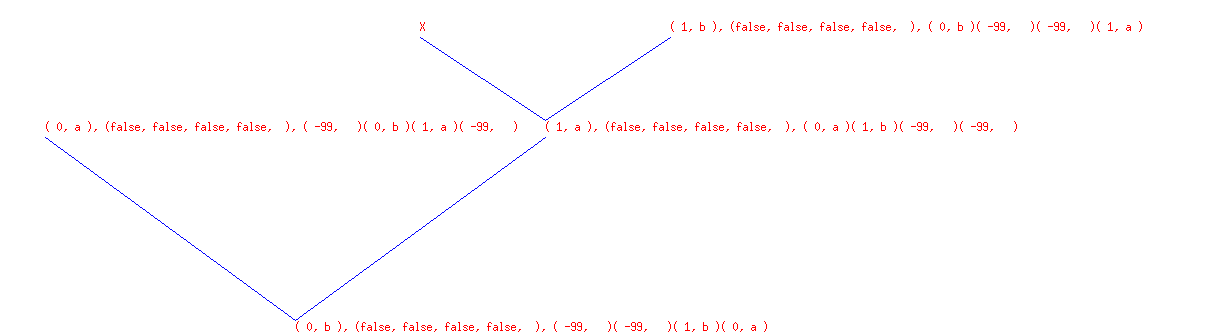
\includegraphics[width=15cm]{images/grid.png}
	\caption{\label{newgrid}Forme de la grille 4x4 apr\`es instantiation}
\end{figure}

\begin{figure}[p]
	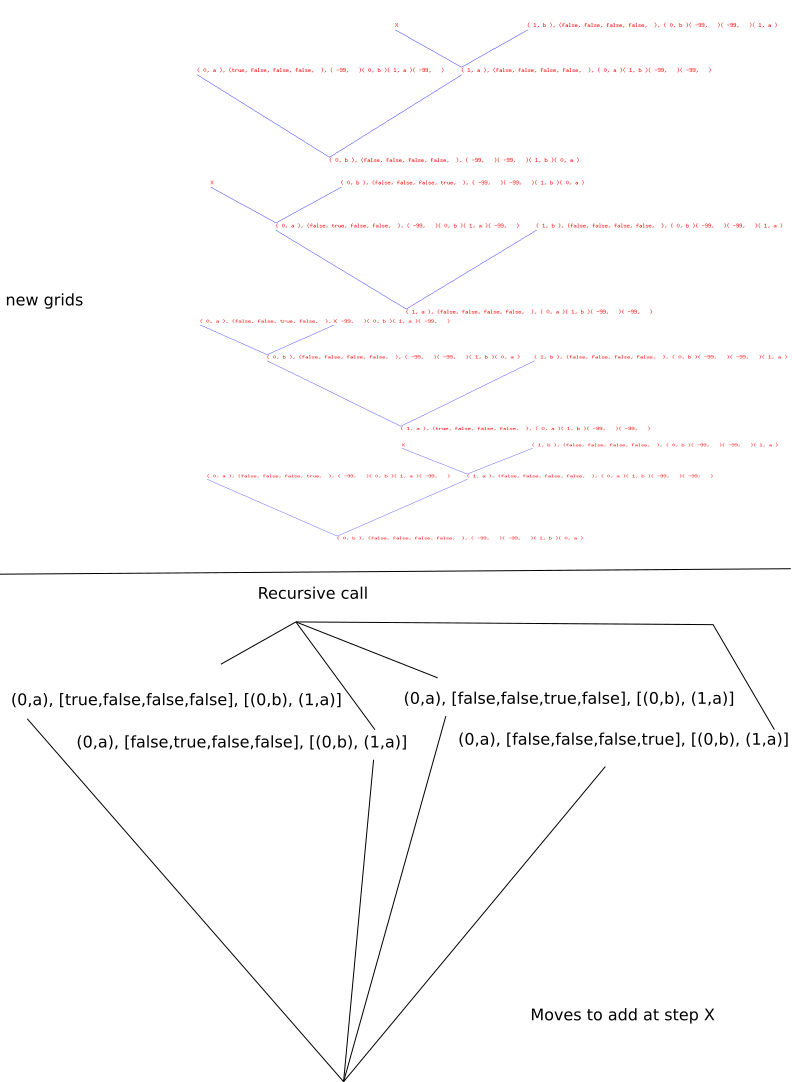
\includegraphics[width=15cm]{images/move_tree_updategrid.png}
	\caption{\label{arbre_possible_updategrid}Noeud \`a ajouter dans l'arbre des possible et grille mise \`a jour pour l'appel r\'ecursif}
\end{figure}

\begin{figure}[p]
	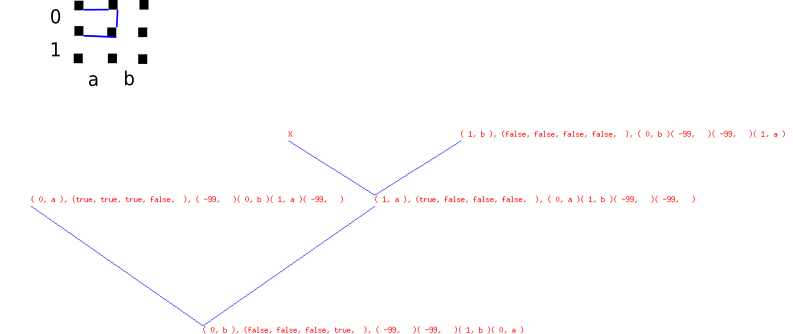
\includegraphics[width=15cm]{images/initialstateplay.png}
	\caption{\label{conf_initiale_jeu}Etat de la grille apr\`es les 3 coups jouers.}
\end{figure}

\begin{figure}[p]
	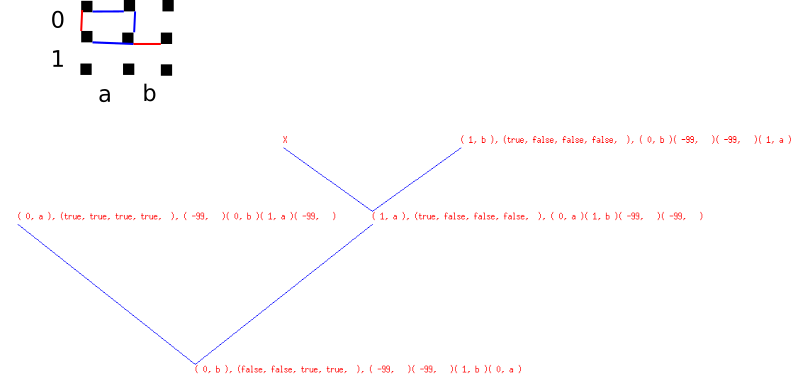
\includegraphics[width=15cm]{images/grid_state_play_ia0.png}
	\caption{\label{ia0plays}Etat de la grille apr\`es que l'IA 0 aie jou\'e.}
\end{figure}

\begin{figure}[p]
	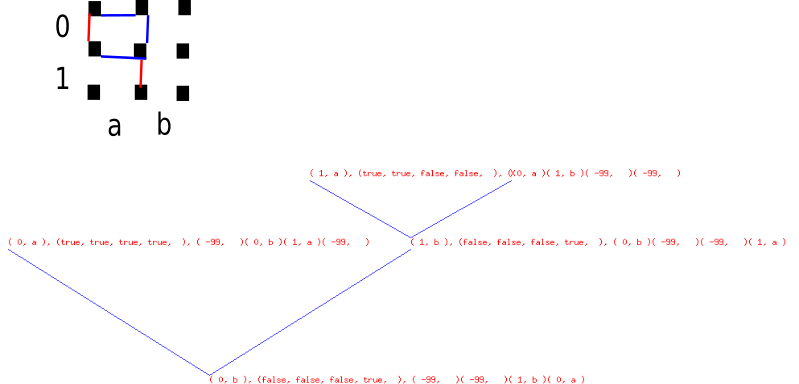
\includegraphics[width=15cm]{images/grid_state_play_ia1.png}
	\caption{\label{ia1plays}Etat de la grille apr\`es que l'IA 1 aie jou\'e.}
\end{figure}

\begin{figure}[p]
	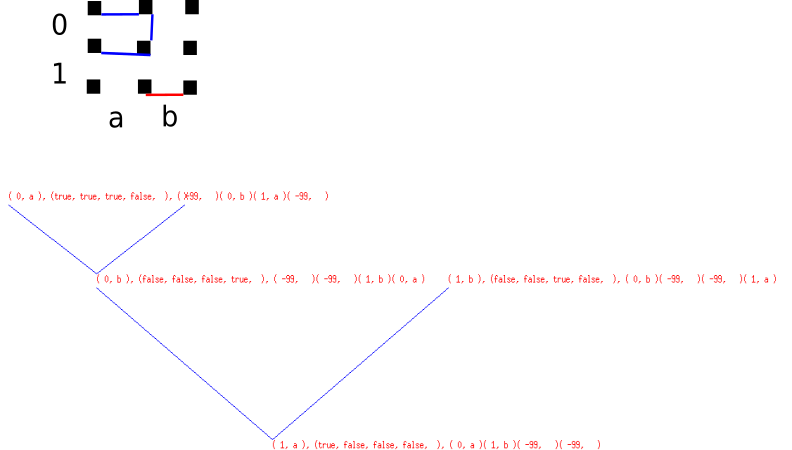
\includegraphics[width=15cm]{images/grid_state_play_ia2.png}
	\caption{\label{ia2plays}Etat de la grille apr\`es que l'IA 2 aie jou\'e.}
\end{figure}


\end{document}
